In this section the KDM-RE is presented. 
In Figure~\ref{fig:process} we depict the overall process of our technique which was adapted based on the horseshoe modernization model. 
It is split into three parts, they are: 
(\textit{i}) Reverse Engineering, 
(\textit{ii}) Refactorings and 
(\textit{iii}) Forward Engineering. 
Furthermore, our process is divided into six levels (\textbf{Level-0} to \textbf{Level-1}), as can be seen in Figure~\ref{fig:process}. 

\subsection{Reverse Engineering}

Firstly, the engineer starts the process in the \textbf{Level-0} by choosing an eclipse project which contains the source-code to realize the refactorings.  
After that, into \textbf{Level-1} the source-code need to be transformed into a Platform-Specific Model (PSM). 
This PSM is an instance of the source-code which represents all abstraction of the source-code. To realize this transformation we implemented a model extractor in Java. To implement this model extractor we carried out three activities: 1) definition of the Java grammar, 2) mapping of Java grammar elements to elements of Java Model, and 3) implementation of the model extractor. For the definition of the Java grammar we used the Xtext\footnote{https://www.eclipse.org/Xtext/} framework. Using this framework we obtained automatically three artifacts: 1) a metamodel, 2) a textual editor and 3) a Java parser that allow us to recognize the elements of the Java grammar from code written in java. 
Figure~\ref{fig:discovery_java_model} illustrates how KDM-RE manages to assist the engineer to get the instance of this PSM. Figure~\ref{fig:discovery_java_model} (a) shows the eclipse project selected by the engineer - then after the engineer click in a popup menu named ``Discovery Java Model'' the Figure~\ref{fig:discovery_java_model} (b) is shown an excerpt to indicate the correspondence with the legacy Java Model.
%This PSM is an Abstract Syntax Tree (AST) that represents the syntactic struct of Java source code.

\begin{figure}[!ht]
\centering
  % Requires \usepackage{graphicx}
  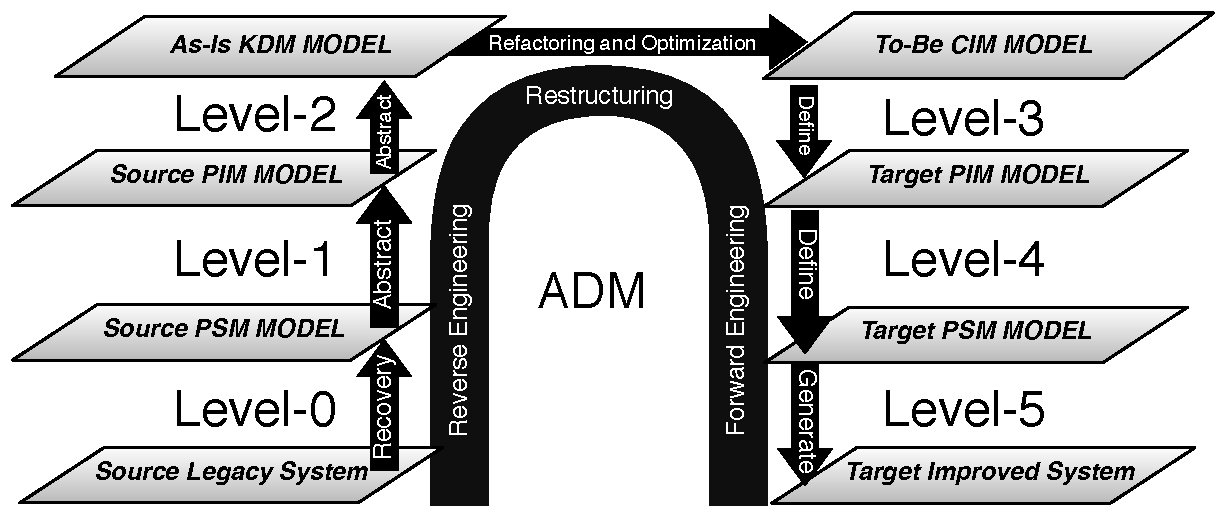
\includegraphics[width=11cm, height=3.8cm]{figure/processoDaFerramenta}
\caption{KDM-RE Process}
\label{fig:process}
\end{figure} 

After creating the PSM the next level (\textbf{Level-2}) consists in transforming the PSM to a Platform-Indented Model (PIM) which is based on the KDM. 
In this level the KDM-RE performs a set of  Model-To-Model (M2M) transformation to get an instance of the KDM which represents the systems ``AS-IS''. 
These transformations are performed by ATL (ATL Transformation Language)\footnote{https://www.eclipse.org/atl/}.
Similarly, the KDM-RE also provides a popup menu named ``Discovery KDM Model'' which by clicking on it the engineer gets a instance of the KDM based on the earlier PSM.
In Figure~\ref{fig:discovery_java_model}(c) shows how the Java Model is transformed to KDM.

\begin{figure}[!ht]
\centering
  % Requires \usepackage{graphicx}
  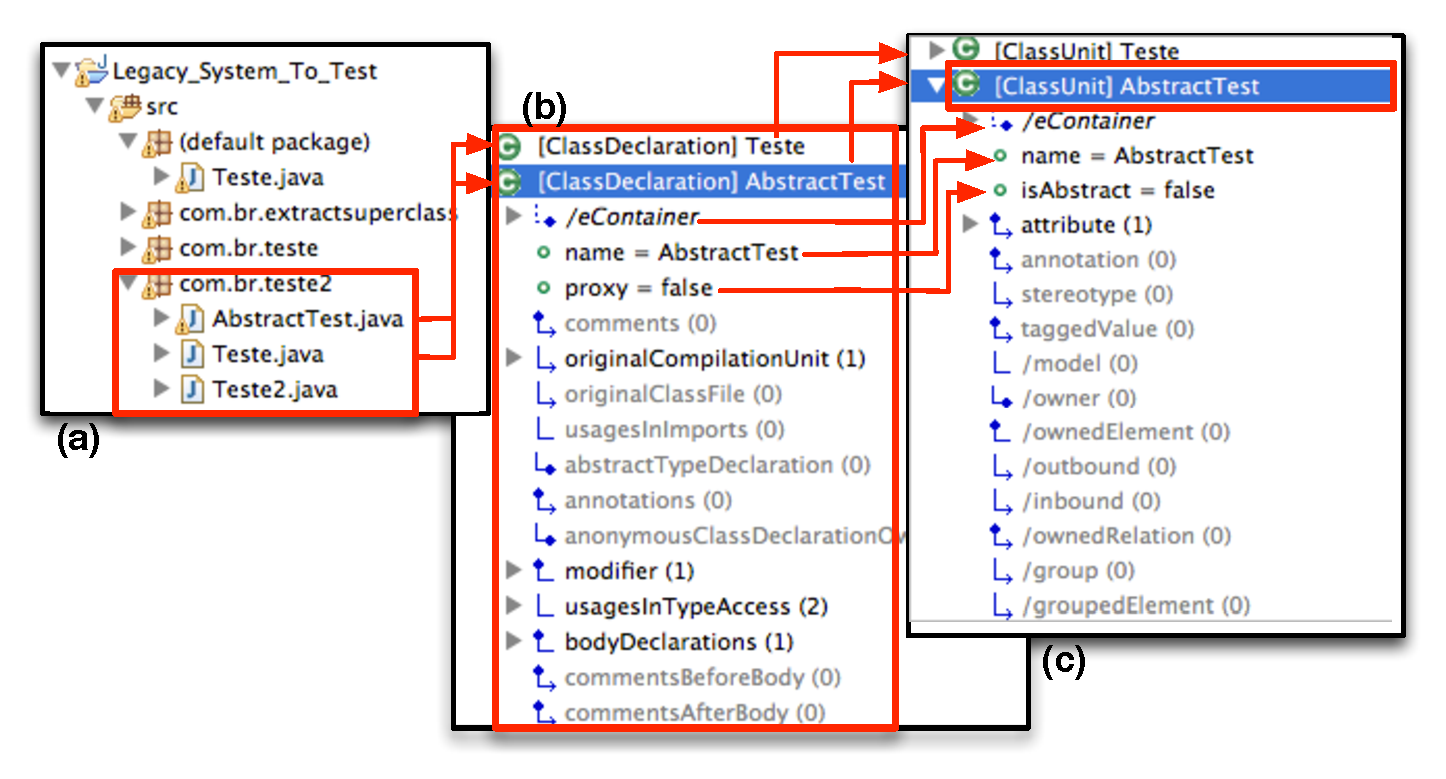
\includegraphics[width=13cm, height=6cm]{figure/GerandoTODOS}
\caption{Process to Discovery Java and KDM Model}
\label{fig:discovery_java_model}
\end{figure}

In Figure~\ref{fig:interface} we depicted the main window of our \textit{plug-in}. 
For explanation purpose, we have identified main regions, i.e., \textcircled{a}, \textcircled{b}, \textcircled{c} and \textcircled{d}.

\begin{figure}[!ht]
\centering
  % Requires \usepackage{graphicx}
  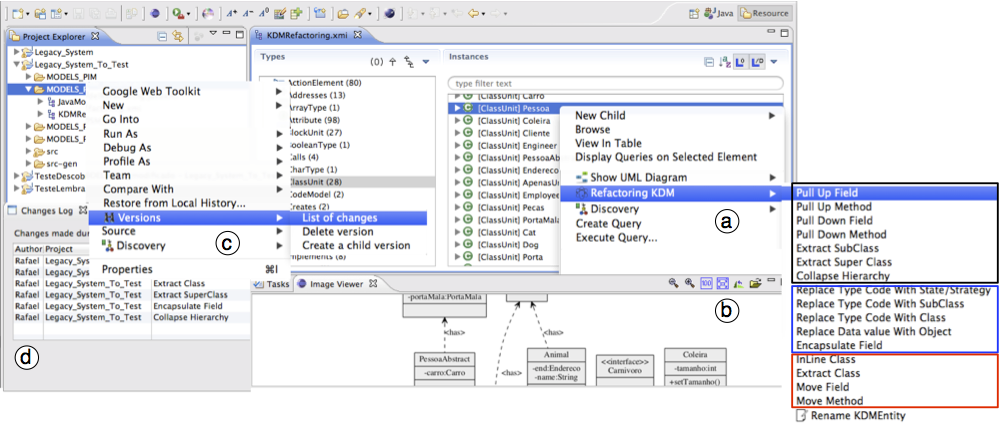
\includegraphics[width=15cm, height=6.8cm]{figure/ScreenShot_tool}
\caption{KDM-RE's Interface}
\label{fig:interface}
\end{figure}

All refactorings provided by KDM-RE are based on the KDM model. 
%Thus, suppose that a KDM model has already been instantiated. 
%All the steps to how obtain a KDM instance are explained further. 
In order to assist the refactorings we extended the KDM's model browser provided by MoDisco\footnote{http://www.eclipse.org/MoDisco/}. 
We added a popup menu named ``Refactoring KDM'' in this model browser, see Figure~\ref{fig:interface}\textcircled{a}.
By using this menu the engineer can interact with the KDM model and choose which refactoring must be carried out in the model.
In the region \textcircled{a} can be seen all 16 refactorings that have been implemented in KDM-RE. 
The start of every refactoring is a engineer action in the Eclipse workbench.
For illustration purposes only we drew rectangles to separate the refactorings into three groups. 
The black rectangle represents refactorings that deal with generalization, the blue rectangle stand for refactorings to organize data and the red one symbolize refactoring to assist the moving features between objects.

The region \textcircled{b} (see Figure~\ref{fig:interface}) shows a class diagram that is generated as the engineer performs the refactorings in KDM model, i.e., changes are reproduced on the fly in a class diagram.
We claim that this is important once the class diagram provides an abstract view of the system, hence, the engineer can visually check the system's changes after applying a set of refactorings. 
In addition, usually the source code is the only available artifact of the legacy software. 
Therefore, creating a class diagram makes, both the legacy software and the generated software to have a new type of artifact (i.e., UML class models), improving their documentation.

KDM-RE also supplies a multiple versions of a system at level models (KDM) which allows the engineer to work interactively on multiple models and to explore alternate refactoring path. As can see in the region \textcircled{c} (see Figure~\ref{fig:interface}), the engineer must select a KDM file, then he must right-click on the mouse to appear a popup menu named ``Versions''. By releasing the mouse on this menu, three options is shown: (\textit{i}) List of changes, (\textit{ii}) Delete version and (\textit{iii}) Create a child version. The last option create a copy of the KDM file - then the engineer can explore another refactoring path. The second option delete a specific version - first option shows all changes that have been realized in a current KDM file, all changes are depicted in an Eclipse View, as shown in region \textcircled{d}. In this View it is possible to visualize the author that have committed the changes, the project and all refactorings realized.


\subsection{Executing Refactoring KDM-RE}

After the engineer clicks on the menu-item (see Figure~\ref{fig:interface} \textcircled{a}) and choose which refactoring to apply, a method run() in the class related to the chosen refactoring is being called. In this method the refactoring classes and a ``RefactoringWizard'' are started. In every refactoring the KDM file must be analyzed to find the meta-classes that are affected by a specific refactoring. Because of the structure of the KDM file, the easiest way to do this, is a traversal using the visitor pattern~\cite{gamma}. Therefore we implemented the visitor pattern in KDM-RE to assist the travel of all meta-classes in a correct order.

\begin{figure}[!ht]
\centering
  % Requires \usepackage{graphicx}
  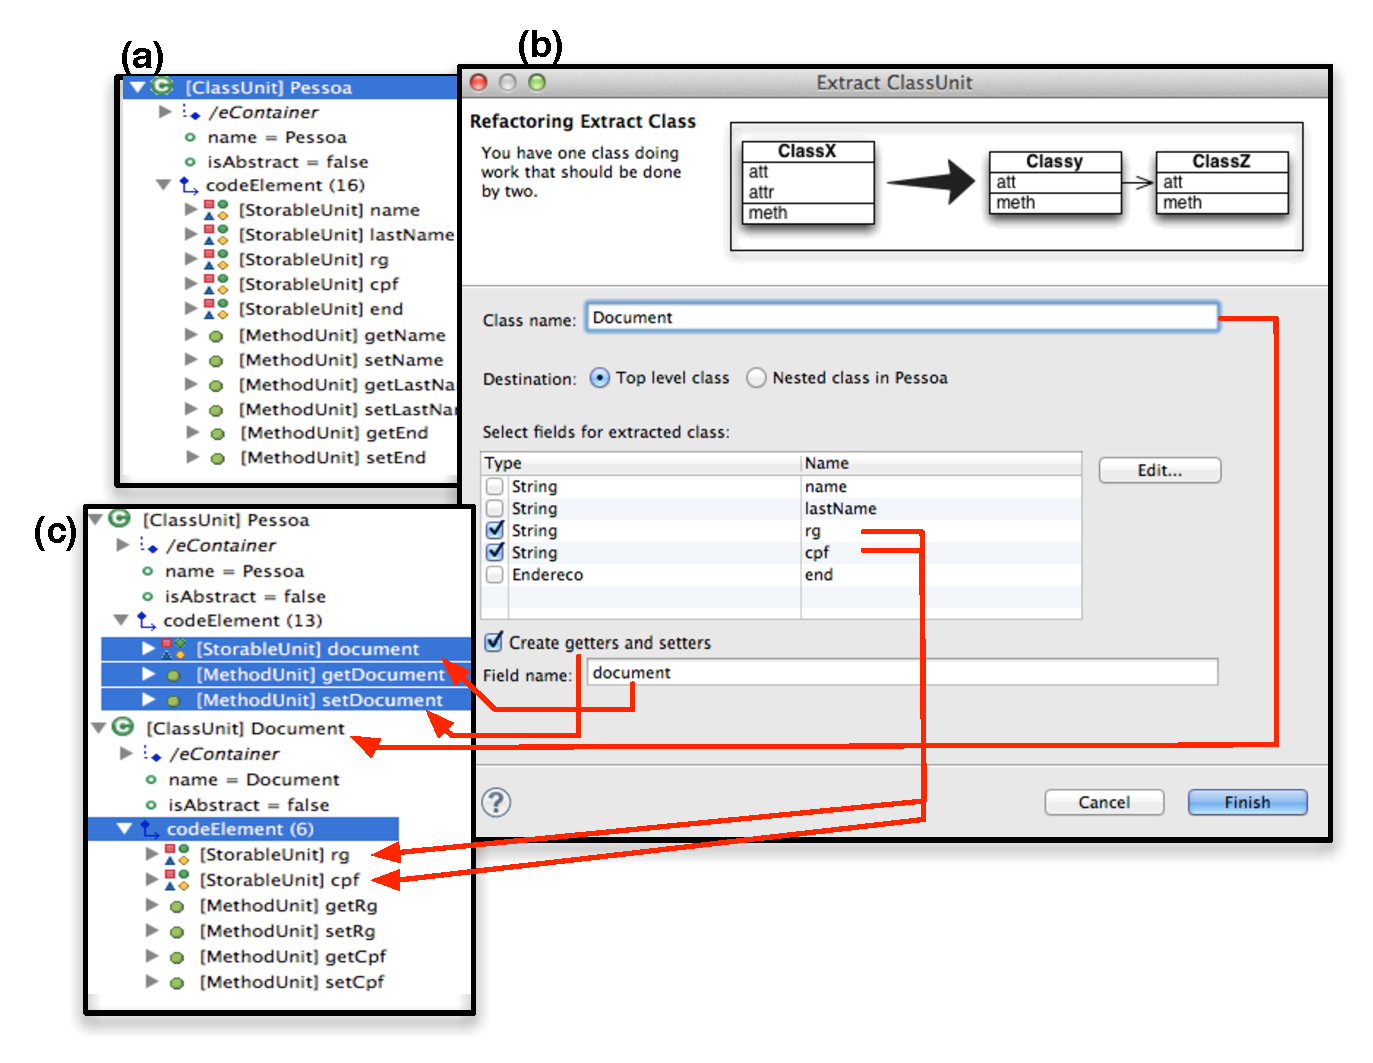
\includegraphics[scale=0.6]{figure/Wizard2}
\caption{Extract Class Wizard}
\label{fig:wizard}
\end{figure}

For explanation purpose pretend that the engineer found out that one class is doing work that should be done by two, thus, he must apply the refactoring ``Extract Class''. As stated earlier the first step is to select the metaclass that should be extracted into a separate one, this step is illustrated in Figure~\ref{fig:wizard}(a). After selecting the metaclass, a right-click opens the context menu where the refactoring is accessible. After the click, the system displays the ``RefactoringWizard'' to the engineer, Figure~\ref{fig:wizard}(b) depicts the Extract Class Wizard. In this wizard, the name of the new metaclass can be set. Also a preview of all detected ``StorableUnits'' and ``MethodUnits'' can be chosen to put into the new metaclass. Further, the engineer can select if either the new metaclass will be a top level metaclass or a nested metaclass. The engineer also can select if the KDM-RE must create instances of ``MethodUnits'' to represent accessors methods (gets and sets). Finally, the engineer can set the name of the ``StorableUnit'' that represent the link between the two metaclasses (the old metaclass and the new one). After all of the required inputs have been made, the engineer can click on the button ``Finish'' and the refactoring ``Extract Class'' is performed by KDM-RE. As can be seen in Figure~\ref{fig:wizard}(c) a new instance of ``ClassUnit'' named ``Document'' was created - two StorableUnit from ``Pessoa'', i.e., ``rg'' and ``CPF'' were moved to the new ``ClassUnit'' - instances of ``MethodUnits'' were also created to represent the gets and sets. In addition, the instance of ``ClassUnit'' named ``Pessoa'' owns a new instance of ``StorableUnit'' that represent the link between both ``ClassUnits''. Due space limitation the other ``StorableUnits'' of ``ClassUnit'' named ``Pessoa'' are not shown in Figure~\ref{fig:wizard}(c).

After the engineer realize the refactoring a UML class diagram is created on the fly to mirror graphically all changes performed in the KDM model, see Figure~\ref{fig:interface}\textcircled{b}. Moreover, the KDM-RE creates/updates a tracking log to show the historic of all changes performed in the system, as can be see in Figure~\ref{fig:interface}\textcircled{d}. 

\subsection{Forward Engineering}
After the engineer realize the refactoring the next steps are to transform the KDM model to a PSM, i.e., a Java Model and to generate the refactored source-code conforming the PSM. The former step is carried out based on a set of transformations using ATL, due space limitation these transformations are not depicted. The latter was performed by using a textual template approach, such as the Acceleo\footnote{http://www.eclipse.org/acceleo/}. A template can be thought of as the target text with holes for variable parts. The holes contain metacode which is run at template instantiation time to compute the variable parts. In Figure~\ref{fig:forward_Engineering} the generation of source code using template is depicted.

\begin{figure}[!ht]
\centering
  % Requires \usepackage{graphicx}
  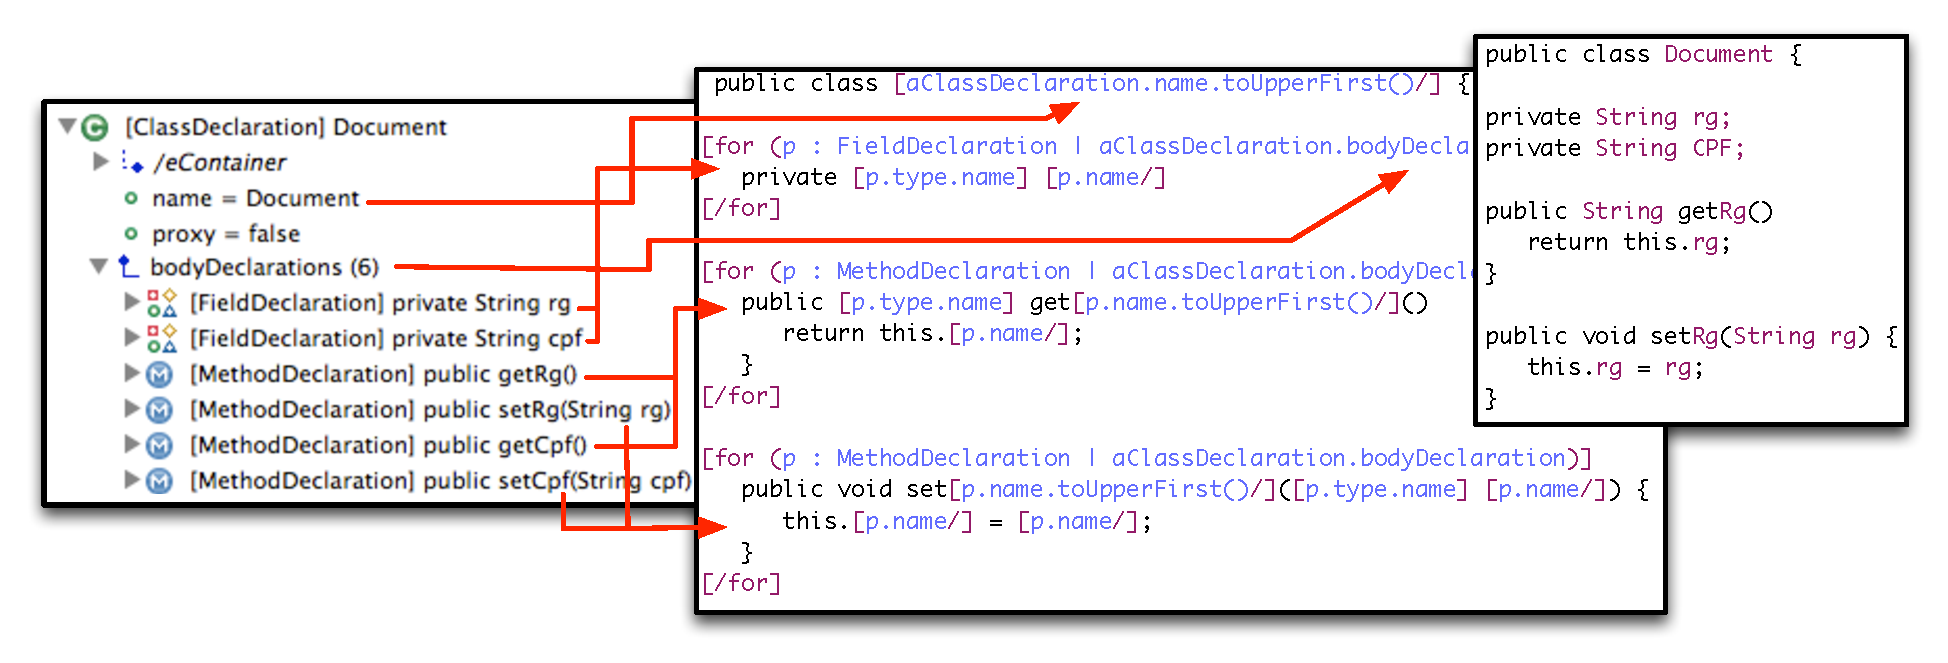
\includegraphics[scale=0.48]{figure/ForwardEngineering}
\caption{Forward Engineering steps}
\label{fig:forward_Engineering}
\end{figure}





to generate Java code from class models conforming to the meta- model in Figure 2(a).



